\usepackage[utf8]{inputenc}
\usepackage[T1]{fontenc}
\usepackage[ngerman]{babel}
\usepackage{avant}
\mode<article>{\usepackage{tgschola}}

\usepackage{listings}

\usepackage{tikz}
\usetikzlibrary{intersections}
\usetikzlibrary{arrows,decorations.pathmorphing,backgrounds,positioning,fit}


\mode<presentation>{\beamertemplatenavigationsymbolsempty}

\usetheme{Laser}

\mode<article>{
\newenvironment{niitemize}{
\begin{itemize}}{\end{itemize}}
}

\makeatletter
\mode<presentation>{
\newenvironment{niitemize}{
  \ifnum\@itemdepth >2\relax\@toodeep\else
      \advance\@itemdepth\@ne%
      \beamer@computepref\@itemdepth%
      \usebeamerfont{itemize/enumerate \beameritemnestingprefix body}%
      \usebeamercolor[fg]{itemize/enumerate \beameritemnestingprefix body}%
      \usebeamertemplate{itemize/enumerate \beameritemnestingprefix body begin}%
      \begin{list}
        {
            \usebeamertemplate{itemize \beameritemnestingprefix item}
        }
        { \leftmargin=1.2em \itemindent=0em
            \def\makelabel##1{%
              {%
                  \hss\llap{{%
                    \usebeamerfont*{itemize \beameritemnestingprefix item}%
                        \usebeamercolor[fg]{itemize \beameritemnestingprefix item}##1}}%
              }%
            }%
        }
  \fi
}
{
  \end{list}
  \usebeamertemplate{itemize/enumerate \beameritemnestingprefix body end}%
}
}
\makeatother

\setbeamercolor{normal text}{fg=black,bg=black!2}

\lstset{
columns=fullflexible,
basicstyle=\ttfamily,
}


\newcommand{\LA}{\ensuremath{\Leftarrow}}
\newcommand{\la}{\ensuremath{\leftarrow}}
\newcommand{\RA}{\ensuremath{\Rightarrow}}
\newcommand{\ra}{\ensuremath{\rightarrow}}
\newcommand{\lra}{\ensuremath{\leftrightarrow}}
\newcommand{\On}{\ensuremath{O(n)}\xspace}
\newcommand{\Ologn}{\ensuremath{O(\log n)}\xspace}
\newcommand{\Oone}{\ensuremath{O(1)}\xspace}

\title{Presslufthammer}
\subtitle{Project Status}
\date{WiSe 2011/12}
\author{Aljoscha Krettek \and Peter Grätz \and Fabian Eichhorn}
\institute
{
  \inst{}
  DIMA\\
  Technische Universität Berlin
}
\subject{Textmining}

\begin{document}

\begin{frame}[t,plain]
\titlepage
\end{frame}

\begin{frame}[t,plain]{Agenda}
\tableofcontents
\end{frame}

\section{Project Overview}

\begin{frame}<presentation>{Project Overview}
\begin{niitemize}
 \item Open source implementation prototype of Google BigQuery, based on Dremel
   paper\footnote{http://research.google.com/pubs/pub36632.html}
 \item Handling of mostly aggregation queries on very large data
 \item Data stored in novel columnar format on cluster of machines
 \item Hierarchy of compute nodes for interactive query performance
 \item SQL-like query language
\end{niitemize}
\end{frame}

\section{Storage}

\begin{frame}<presentation>{Hierarchical vs. Columnar}
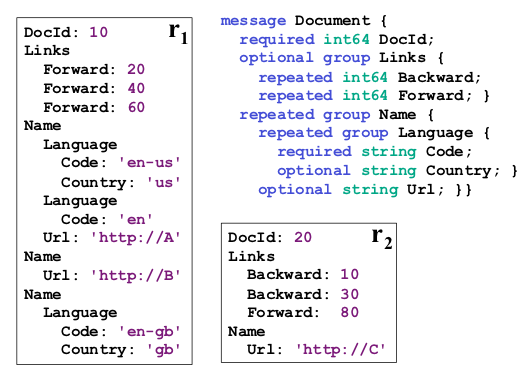
\includegraphics[width=.49\textwidth]{gfx/hierarchical-schema}
\hfill
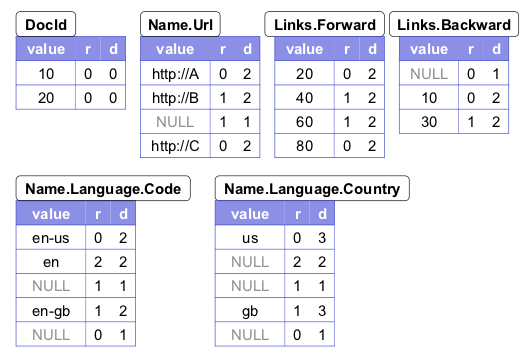
\includegraphics[width=.5\textwidth]{gfx/columnar}

\begin{niitemize}
 \item Repetition/Definition levels represent record structure
 \item \texttt{FieldStriper} stripes records to columns
 \item \texttt{AssemblyFSM} assembles records from columns
\end{niitemize}
\end{frame}

\begin{frame}<presentation>{Record Striping}
\begin{niitemize}
 \item Recursively stripe record from a \texttt{RecordStore} using a
  \texttt{RecordDecoder} and tree of \texttt{FieldWriter}S
 \item Implementation of \texttt{RecordStore} and \texttt{RecordDecoder} only
  for JSON for now
 \item Data written to a \texttt{Tablet} using a \texttt{ColumnWriter}
 \item Implementation of \texttt{ColumnWriter} and \texttt{Tablet} for on-disk
  storage and in-memory so far
\end{niitemize}
\end{frame}

\begin{frame}<presentation>{Record Assembly}
\begin{niitemize}
 \item Assemble records to a \texttt{RecordStore} using a
  \texttt{RecordEncoder} using \texttt{AssemblyFSM}
 \item Read columnar data from \texttt{Tablet} using a \texttt{ColumnReader}
\end{niitemize}

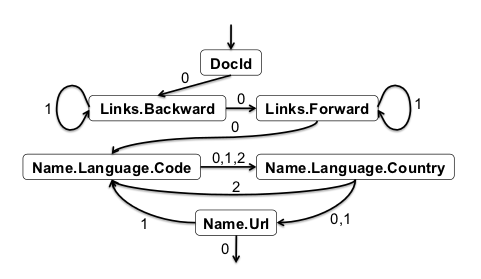
\includegraphics[width=.49\textwidth]{gfx/full-assemblyfsm}
\hfill
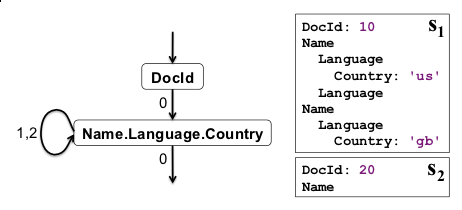
\includegraphics[width=.49\textwidth]{gfx/partial-assemblyfsm}
\end{frame}

\begin{frame}<presentation>{Issues}
\begin{niitemize}
 \item Data format difficult to understand, sometimes descriptions
  in paper inconsistent
 \item ``Algorithms'' in paper for striping, assembly and query processing are only
  rough sketch, still required lot of
  thinking/debugging
\end{niitemize}
\end{frame}

\section{Query Execution}
\begin{frame}<presentation>{Query Execution}
\begin{niitemize}
 \item Only projection for now
 \item Uses columnar data throughout, only last result as
  records (hierarchical) to client
 \item Columnar data read from source tablet into target tablet, ignoring
  columns that are projected out
\end{niitemize}
\end{frame}

\begin{frame}<presentation>{Issues}
\begin{niitemize}
 \item Query processing only sketched in paper, only basic
  select-project-aggregate
\end{niitemize}
\end{frame}

\section{Network}
\begin{frame}<presentation>{Network}
  Dremel architecture consists of four types of nodes
  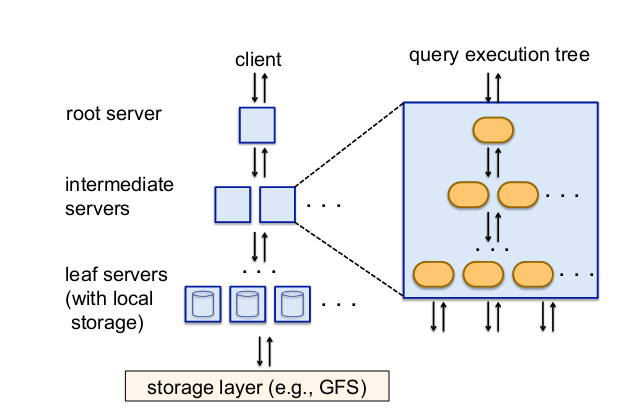
\includegraphics[width=.55\textwidth]{gfx/net-arch}
  \begin{niitemize}
    \item Coordinator
    \item Inner
    \item Leaf and
    \item Client Nodes
  \end{niitemize}
\end{frame}

\begin{frame}<presentation>{Coordinator and Inner Nodes}
  Coordinator Node
  \begin{niitemize}
    \item Accepts Queries from Clients
    \item Parses Queries
    \item Hands Out Jobs to Leafs
  \end{niitemize}
  Inner Nodes
  \begin{niitemize}
    \item Not Implemented
    \item Build an intermediate layer
    \item Take care of splitting/aggregating queries
  \end{niitemize}
\end{frame}

\begin{frame}<presentation>{Leaf and Client Nodes}
  Leaf Node
  \begin{niitemize}
    \item Connection between Network and Storage
    \item Data fetching / Storage Access
    \item Per Tablet Query processing
  \end{niitemize}
  Client Node
  \begin{niitemize}
    \item Provides the UI
    \item Attaches to a Coordinator
    \item Only basic CLI version implemented
  \end{niitemize}
\end{frame}


\begin{frame}<presentation>{Issues}
\begin{niitemize}
 \item Coordination of Nodes: Intermediate Layer
 \item Proper Serialization of Meta-Data for Transfer
\end{niitemize}
\end{frame}



\section{TODO}
\begin{frame}<presentation>{TODO}
\begin{niitemize}
 \item Write unittests for a lot of things to be confident that changes
  do not break things
 \item Maybe add a proper storage layer
 \item Revisit the striping/assembly algorithms
 \item Implement proper query handling using a pseudo-SQL language
 \item Probably rethink networking code, implement real network
  topology (root, inner nodes, leafs)
 \item Code generation for query processing
\end{niitemize}
\end{frame}

\end{document}
